\documentclass{article}

\usepackage{amsmath}
\usepackage{amsfonts}
%\usepackage{amssymb}
\usepackage{graphicx}
\usepackage{float}
\usepackage[autostyle]{csquotes}
\usepackage{acronym}
\usepackage{babel}
\usepackage{url}
\usepackage{algorithm}
\usepackage[noend]{algpseudocode}
\usepackage{tikz}
\usepackage{tabularx}
\usepackage{array}
\usepackage{subfig}

\usepackage[style=nature]{biblatex}
\addbibresource{sources.bib}

\newcolumntype{L}{>{\raggedright\arraybackslash}p}
\newcommand{\re}[1]{\textbf{\textcolor{orange}{#1}}}
\newcommand{\add}[1]{\textbf{\textcolor{blue}{#1}}}


\title{
	A systematic comparison of different methods to analyse COVID-19 transmission using graph networks\\
	Expose - tentative title	
}

\author{Simon Westfechtel}

\begin{document}
	\maketitle

	\section{Introduction}
	\label{sec:Introduction}
	When news of a novel coronavirus, latter dubbed coronavirus disease 2019, or COVID-19, first emerged from the People's Republic of China in late 2019, there was a lot of uncertainty regarding its danger potential. Especially in western countries, governments warned about 'fake news' and downplayed the severity of the virus, e.g. discouraging the purchase of protective face masks \cite{osthessen_news,tagesschau_1,tagesschau_2}. After the epidemic character of the disease had become apparent, the focus soon shifted to slowing or halting the spread of the virus. The efficient tracing of infected individuals' social contacts plays an integral part in preventing the spreading of a disease, and had been a well-established procedure well before the emergence of COVID-19, where for instance a verified case of tuberculosis requires a notification of the health departments \cite{enwiki_1097839709}. 
	
	While a known and tested method, the sheer number of cases soon threatened to overwhelm healthcare systems and health departments alike. In order to prevent this worst-case scenario, it became paramount to identify sources of infection and transmission chains. Where medical research focused primarily on virological factors (e.g. which individual features would predispose someone to infection and/or a severe course of illness, how the virus is transmitted from person to person, etc.), the field of computational social sciences offers a different approach. 
	
	Although contact tracing initiatives differ in the level of detail that is being recorded, in general they at least identify the source of infection, i.e. a symptomatic or, once tests had become widely available, positively tested patient being reported to the local health department, and said patient's social contacts, i.e. the people who had come into contact with the patient prior to being aware of the infection, and who thus could have been infected themselves, and possibly spread the virus further (i.e. the transmission chain). 
	
	With this information alone, it is possible to model transmission chains as social networks \cite{hainan_publication,shanxi_publication,hancean2022occupations}, where individuals constitute the set of vertices, and contacts between individuals are represented by edges between the respective nodes; for an illustration, refer to figure \ref{fig:example_case_network}. Thus, through the usage of methods of social network analysis, it becomes possible to identify dynamics in the spread of the virus which might otherwise have been overlooked. Additionally, if further information like age, health status and profession were also collected during the contact tracing procedure, modern machine learning approaches can reliably identify covariates that influence the viral spread (e.g. whether younger people are more likely to get infected and/or infect others compared to other age groups).
	
	\begin{figure}
		\centering
		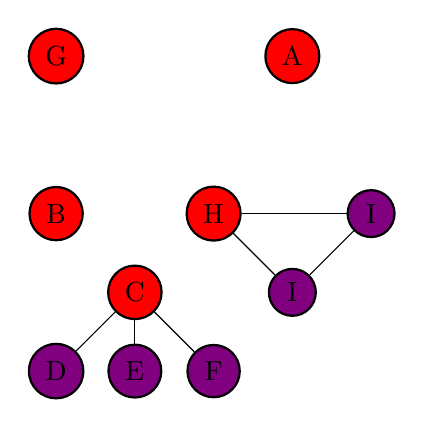
\begin{tikzpicture}
			\begin{scope}[every node/.style={circle,thick,draw,fill=red}]
				\node (A) at (2,2) {A};
				\node (B) at (-1,0) {B};
				\node (G) at (-1,2) {G};
				\node (C) at (0,-1) {C};
				\node (H) at (1,0) {H};
			\end{scope}
		
			\begin{scope}[every node/.style={circle,thick,draw,fill=violet}]
				\node (D) at (-1,-2) {D};
				\node (E) at (0,-2) {E};
				\node (F) at (1,-2) {F};
				\node (I) at (3,0) {I};
				\node (J) at (2,-1) {I};
			\end{scope}
		
			\begin{scope}
				\path (C) edge node {} (D);
				\path (C) edge node {} (E);
				\path (C) edge node {} (F);
				\path (H) edge node {} (I);
				\path (H) edge node {} (J);
				\path (I) edge node {} (J);
			\end{scope}
		\end{tikzpicture}
		\caption{Exemplary case contact network. Confirmed cases are coloured red, and reported contacts are coloured purple.}
		\label{fig:example_case_network}
	\end{figure}
	
	\section{Related work}
	\label{sec:Related_work}
	As one would expect, there is ample scientific work on the topic of COVID-19, and the same goes for case contact networks. Typically, case reports from health authorities are translated into a social network structure, which is then analysed using established methods from computer science. These include, but are not limited to:
	\begin{itemize}
		\item Degree centrality: A centrality measure which is equivalent to the node's degree (sometimes expressed on a [0,1] scale), where a higher value indicates a more central node \cite{golbeck}. Here, it is used as an indicator for the transmission rate of individual cases, i.e. how many people they infect \cite{hainan_publication,shanxi_publication}.
		\item Betweenness centrality: A centrality measure which measures the number of shortest paths that go through the node in question, where higher values indicate nodes that facilitate the flow of information \cite{golbeck}. Here, it is also used to determine a patient's influence on transmitting the virus \cite{hainan_publication}.
		\item PageRank score: A centrality measure based on eigenvector centrality. It is computed by performing random walks on the network and measuring for each node the likelihood to arrive at that node, i.e. a higher score is assigned to nodes which are frequently pointed at \cite{gleich_pagerank}. Here, it is used to determine a patient's position in the overall network \cite{hainan_publication,shanxi_publication}.
		\item Community detection: Communities in a network context may be defined in various ways; generally, the task of community detection is dividing the graph into a set of subgraphs according to specific criteria. Here, this division is based on network cohesion, i.e. the nodes making up a subgraph should be strongly interconnected, which is also known as a \emph{connected component}; in other words, the connected components are equivalent to the network's communities (achieved e.g. by \emph{Markov clustering algorithm} \cite{community_detection,markov_clustering}). In the context of this work, it is used to investigate infection dynamics \cite{hainan_publication}.
		\item Triadic structure: A measure for network structure. For any triplet of nodes $(v_1,v_2,v_3)$, or triad, there are exactly eight possible edge configurations (assuming an undirected graph): 
		\begin{align*}
			&\emptyset,\{(v_1,v_2)\},\{(v_2,v_3)\},\{(v_1,v_3)\},\{(v_1,v_2),(v_2,v_3)\},\{(v_1,v_2),(v_1,v_3)\},\\ &\{(v_1,v_3),(v_2,v_3)\},\{(v_1,v_2),(v_2,v_3),(v_1,v_3)\}
		\end{align*}
		Investigating triadic structure may yield insights into the relationship of network cohesion and network density \cite{triadic_effects}. Here, it is used to investigate the spread pattern of the virus \cite{shanxi_data}.
	\end{itemize}
	
	\noindent Although useful information can already be extracted from the data using aforementioned methods, they have two main shortcomings. First, the raw data is (ideally) structured in a time-stamp format, i.e. case information includes the date when they were reported to/recorded by the health authorities. Since most previous work on this topic ignores this temporal aspect and case contact data is modelled as static networks where interaction between actors takes the form of relational states as opposed to relational events (e.g. "Actor A is contact of Actor B" vs. "Actor A came into contact with Actor B on date D"), other methods might be better suited to analyse data of this kind. Relational event models, or REMs \cite{perry2013point,butts20084}, are a promising approach to this type of data. They can be used to discover various patterns in actor interactions and discover these patterns' influence on future interactions, e.g. whether similar actors are more likely to interact (homophily) \cite{butts20084,pilny_rem}, or whether prior transitive interactions between actors (i.e. actors are indirectly connected) increase the likelihood for a direct future interactions (transitive closure) \cite{butts20084}.
	
	While this is a great improvement over static models, relational event models, or REMs, only consider dyadic interaction, i.e. for any interaction, only two actors are considered, i.e. interactions are assumed to be dyadic; in reality, however, interactions often involve multiple actors, which is especially true for disease transmission, e.g. a COVID-positive individual coming into contact with customers and staff while grocery shopping. Thus, modelling such interactions in a dyadic way might miss key insights. Common ways to alleviate this shortcoming are treating all dyads stemming from a polyadic interaction as independent, or clustering all targets of the interaction into a single multi-actor node \cite{butts20084,perry2013point}; refer to figure \ref{fig:polyadic_interactions} for an illustration.
	
	\begin{figure}
		\hspace*{\fill}
		\subfloat[Method 1: Model receiver set as a single node.]{
			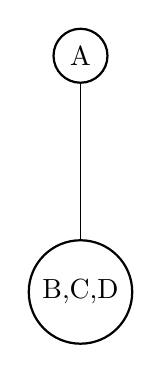
\begin{tikzpicture}
				\begin{scope}[every node/.style={circle,thick,draw}]
					\node (A) at (0,0) {A};
					\node (B) at (0,-3) {B,C,D};
				\end{scope}
				
				\begin{scope}
					\path (A) edge node {} (B);
				\end{scope}
			\end{tikzpicture}
		}
		\hfill
		\subfloat[Method 2: Model one edge for each node of the receiver set. Edges are assumed to be independent.]{
			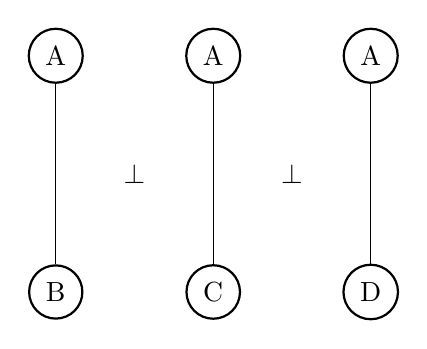
\begin{tikzpicture}
				\begin{scope}[every node/.style={circle,thick,draw}]
					\node (A1) at (0,0) {A};
					\node (A2) at (2,0) {A};
					\node (A3) at (4,0) {A};
					\node (B) at (0,-3) {B};
					\node (C) at (2,-3) {C};
					\node (D) at (4,-3) {D};
				\end{scope}
			
				\begin{scope}
					\node[draw=none] (A1A2) at (1,0) {};
					\node[draw=none] (BC) at (1,-3) {};
					\node[draw=none] (A2A3) at (3,0) {};
					\node[draw=none] (CD) at (3,-3) {};
				\end{scope}
			
				\begin{scope}
					\path (A1) edge node {} (B);
					\path (A2) edge node {} (C);
					\path (A3) edge node {} (D);
					\path (A1A2) edge[draw=none] node {$\perp$} (BC);
					\path (A2A3) edge[draw=none] node {$\perp$} (CD);
				\end{scope}
			\end{tikzpicture}
		}
		\hspace*{\fill}
		\caption{Two ways to approximate polydiadic interactions.}
		\label{fig:polyadic_interactions}
	\end{figure}
	
	Of course, these methods are only approximations and may fail to accurately represent reality, as well as be unfeasible or even intractable to model \cite{lerner2021relational}. Relational hyperevent models \cite{lerner2021relational,lerner2019rem} build on relational event models and introduce hyperedges, which may connect any number of nodes. Again referring to the above mentioned example of a patient transmitting a virus to multiple people while grocery shopping, this actor would be connected through a hyperedge to the set of infected customers and personnel. Thus, RHEMs make it possible to discover higher-order dependencies present in the data which might be missed by purely dyadic network models like REMs, and therefore produce accurate estimations of network effects \cite{lerner2019rem}. Examples for effects that might be discovered are \emph{receiver set homophily}, i.e. to which degree actors in the receiver set (continuing with the example, infected customers and personnel) share similar attributes, or again triadic effects like transitive closure \cite{lerner2021relational}. Previous work by Lerner et al \cite{lerner2021relational}, where relational hyperevent models have been applied to email data of the Enron company, show RHEMs outperform comparable dyadic methods in terms of model fit and predictive performance. Recently, RHEMs were used by Hâncean et al \cite{hancean2022occupations} to model and analyse a case contact dataset from Bucharest, Romania, showing relational hyperevent models can be utilised to effectively investigate transmission chains in the on-going pandemic.
	\section{Objectives and research questions}
	\label{sec:Research_questions}
	\paragraph{Objective} apply (A) static network models, (B) relational event models, and (C) relational hyperevent models to COVID-19 case contact data. More precisely, (1) identify relevant covariates, (2) analyse influence of covariates on virus transmission, (3) analyse influence of network effects on virus transmission, (4) determine model fit to the data, and (5) determine predictive performance (where applicable).
	\paragraph{Research questions} With the above results, answer the following research questions:
	\begin{enumerate}
		\item Which (1,2) covariates and (3) network effects have a significant influence on the dynamic of virus transmission?
		\item How do (A) static network models, (B) relational event models and (C) relational hyperevent models compare against each other in terms of (4) model fit and (5) predictive performance?
		\item How do case contact networks from different regions compare against each other? Are results generalisable or are the regional differences too great to justify drawing conclusions concerning the overall dynamic of the pandemic?
	\end{enumerate}
	
	\section{Data exploration}
	\label{sec:Data_exploration}
	The basis of this research comprises of four case contact datasets from the People's Republic of China, three of which are smaller, regional sets from the provinces of Yunnan, Hainan and Shanxi, and one larger set from all of China. The regional datasets have already been analysed by Yang et al \cite{hainan_publication,shanxi_publication} using static network models, while the larger dataset has, to the knowledge of the author, not been analysed in the context of social networks so far. In the following, an exploratory summary of the data will be presented.
	
	\paragraph{Yunnan dataset} This dataset contains COVID case information from the province of Yunnan in southern China \cite{hainan_data}. There are 171 entries, with dates ranging from 2020-01-17 to 2020-02-16, i.e. this dataset is from the very early stages of the pandemic. Covariates deemed to be relevant to this research are listed in table \ref{tab:yunnan_hainan_covariates}.
	\begin{table}
		\begin{minipage}{.45\linewidth}
			\begin{tabularx}{\linewidth}{L{.4\linewidth}L{.6\linewidth}}
				\hline
				\textbf{Covariate} & \textbf{Description}\\
				\hline
				Date & Date when the case was confirmed/reported\\
				Gender & Male/Female\\
				Age & In years\\
				Relatives & Whether the patient is a relative of previously recorded cases\\
				\hline
			\end{tabularx}
			\caption{Relevant covariates for the Yunnan and Hainan datasets}
			\label{tab:yunnan_hainan_covariates}
		\end{minipage}
		\hfill
		\begin{minipage}{.45\linewidth}
			\begin{tabularx}{\linewidth}{L{.4\linewidth}L{.6\linewidth}}
				\hline
				\textbf{Covariate} & \textbf{Description}\\
				\hline
				Date & Date when the case was confirmed/reported\\
				Gender & Male/Female\\
				Age & In years\\
				Hukou & Place of residence\\
				Relatives & Whether the patient is a relative of previously recorded cases\\
				\hline
			\end{tabularx}
			\caption{Relevant covariates for the Shanxi dataset}
			\label{tab:shanxi_covariates}
		\end{minipage}
		\begin{tabularx}{\linewidth}{L{.4\linewidth}L{.6\linewidth}}
			\hline
			\textbf{Covariate} & \textbf{Description}\\
			\hline
			Date & Date when the case was confirmed/reported\\
			Gender & Male/Female\\
			Age & In years\\
			Place of residence & \\
			Virus type & Virus variant (e.g. Delta)\\
			Occupation & \\
			Place and event & Activity where infection might have happened\\
			Venue & Location where infection might have happened (e.g. School, Workplace)\\
			With whom & Who might have been the source of infection\\
			Symptom & The patient's symptoms\\
			Symptom severity & \\
			\hline
		\end{tabularx}
		\caption{Relevant covariates for the China dataset}
		\label{tab:china_covariates}
		\begin{tabularx}{\linewidth}{XXXXXX}
			\hline
			\textbf{Dataset} & \textbf{Age} & \textbf{Gender} & \textbf{Residence} & \textbf{Relatives} & \textbf{Degree}\\
			\hline
			Yunnan & $41\pm18$ & $\approx$ & - & $0.51$ & $1.3\pm3.2$\\
			Hainan & $48\pm17$ & $\approx$ & - & $0.46$ & $1.5\pm1.8$\\
			Shanxi & $46\pm16$ & $>men$ & Xian & $0.37$ & $0.99\pm1.3$\\
			China & $42\pm18$ & $>men$ & Xian & - & $3.6\pm18$\\
			\hline
		\end{tabularx}
		\caption{Comparison of covariates between datasets (where applicable). \emph{Gender} states which sex is more common, or whether they are roughly equal. \emph{Residence} is the most common value. \emph{Relatives} specifies the ratio of cases where relatives were recorded previously.}
		\label{tab:cov_comp}
	\end{table}
	114 cases have no ties at all, 25 have one tie, eleven have two ties, six have three ties, two have four and five ties, respectively, and 13 have 12 ties. An average degree of $1.3\pm3.2$ and a median degree of 0 suggest the corresponding contact network is very sparse. Only three of 18 connected components comprise of more than three nodes, suggesting transmission chains were effectively broken to prevent further spread \cite{hainan_publication}. 58 and 62 cases are female and male, respectively; there is no information on gender for 51 patients. This suggests neither sex is more susceptible to the virus. The average age is $41\pm18$ and the median age is 40; with the 75 percentile being 54, patients seem to be mostly younger or middle-aged. 31 out of 60 cases are family members of previously recorded cases; this information is not available for the remaining 111 data records.
	
	\paragraph{Hainan dataset} This dataset contains COVID case information from the province of Hainan \cite{hainan_data}, which is the southernmost province of China. There are 162 entries, with dates ranging from 2020-01-22 to 2020-02-14, i.e. this dataset is also from the early stages of the pandemic. Relevant covariates are the same as for the Yunnan data, listed in table \ref{tab:yunnan_hainan_covariates}. 71 cases have no ties at all, 27 have one tie, 21 have two and three ties, respectively, six have four ties, and eight have five and six ties, each. An average degree of $1.5\pm1.8$, a median degree of 1 and only 43\% of patients without ties compared to 67\% for the Yunnan dataset suggest this network is slightly more dense. Ten out of 27 connected components are comprised of more than three nodes, meaning that in this network, infections are happening in larger clusters and containment methods might not have been as effective. 84 and 78 cases are female and male, respectively; this supports the hypothesis that neither sex is more susceptible to an infection. An average age of $48\pm17$, a 25 percentile of 36, a median age of 51 and a 75 percentile of 62 mean that the patients in this dataset are from an older age group compared to the Yunnan data. 75 out of 162 patients are family members of previously recorded cases.
	
	\paragraph{Shanxi dataset} This dataset contains COVID case information from the province of Shanxi in northern China \cite{shanxi_data}. There are 237 entries, with dates ranging from 2020-01-23 to 2020-02-16, so this dataset too is from the early stages. Relevant covariates mostly correspond to those of the previous two discussed sets, with the addition of the place of residence; they are listed in table \ref{tab:shanxi_covariates}. 108 cases have no tie at all, 68 have one tie, 36 have two ties, 20 have three ties, two have four ties, and three have six, nine or eleven ties, each. An average degree of $.99\pm1.3$, a median degree of 1 and a 45\% no-tie to tie ratio make this dataset and the Yunnan network comparable in density. 12 out of 40 connected components are comprised of more than three nodes, placing this network between the previously discussed networks in terms of infection spread. With 129 versus 108, there are slightly more men in this dataset, albeit not statistically significant. The average age of patients is $46\pm16$, the 25 percentile is 35, the median is 45 and the 75 percentile is 59. Only 87 of the 237 patients are family members of previously recorded cases, suggesting that the majority of infections were transmitted from stranger to stranger. The three most common places of residence are \emph{Xian}, \emph{Ankang} and \emph{Hanzhong}.
	
	\paragraph{China dataset} This dataset contains COVID case information from all of China \cite{china_publication,china_data}. There are 26961 entries (subject to change, depending on possible further preprocessing), with dates ranging from 2020-01-01 to 2022-08-14; therefore, this set stretches over most of the pandemic (as of writing this). Relevant covariates are listed in table \ref{tab:china_covariates}. In contrast to the former datasets, this one contains quite a few more that might yield interesting insights into infection dynamics. 2012 cases have no tie at all, 6179 have one tie, 12818 have two ties, 3194 have three ties, 1619 have four ties, 966 have five ties, 504 have six ties and 2237 cases have more than six ties. 1333 out of 3573 connected components are comprised of more than three nodes. An average degree of $3.6\pm18$, a median degree of 2 and only 2012 cases with no ties mean this network is significantly denser compared to the ones discussed previously. The mean age of patients is $42\pm18$, the 25 percentile is 30, the median is 41 and the 75 percentile is 54, meaning this dataset contains members of all age groups. There is no information on age for 6915 cases. 9218 women versus 11414 men shows a slight bias towards men; 6329 entries contain no information on sex. The three most common occupations are \emph{student} (970), \emph{worker} (548) and \emph{employee} (326). The three most common places of residence are \emph{Xi'an in Shanxi} (1984), \emph{Wuhan in Hubei} (1715) and \emph{Shijiazhuang in Hebei} (888). Where information was recorded, 462 cases have the Delta and 139 cases the Omicron variant. Among the most common activities suspected to be linked to the infection are \emph{travel to Wuhan} (635), \emph{dinner} (359) and \emph{residence in Wuhan} (337). Infections mostly happened during a family gathering (938), outdoors (791) and in a social setting (503). Sources of infection include confirmed cases, family members and \emph{Wuhan personnel}.
	
	\section{Preliminary methods for analysis and evaluation}
	\label{sec:Methods}
	The Hainan, Shanxi and Yunnan datasets mentioned in section \ref{sec:Data_exploration} have all been analysed by Yang et al \cite{hainan_publication,shanxi_publication}, using non event-based approaches. Thus, it seems prudent to analyse these datasets again using relational (hyper-)event models, and compare results in terms of network effects, identifiable covariates and model fit. As all of these datasets are already available in a network format, no special preprocessing steps are necessary. 
	
	The larger dataset comprised of data from the whole of China has, to the knowledge of the author, not yet been analysed in a network context. Therefore, this data should be analysed using all of the methods discussed so far. Results can be compared to the other datasets discussed in section \ref{sec:Data_exploration}. It is worth noting that the coding of the dataset is quite unstructured and at times inconsistent, which might warrant further preprocessing in addition to the preliminary preprocessing already done.
	
	The results produced by the relational (hyper-) event models should further be compared to the results presented by Hâncean et al \cite{hancean2022occupations}, since their work made use of this exact method in a similar context. In this regard, it could be especially interesting to see how transmission dynamics compare between different regions of the world (in this instance, China and Romania). 
	
	Relational event and -hyperevent models will most likely be implemented using the \emph{eventnet} R package \cite{eventnet}, but may necessitate some modifications. Analysis making use of non relational-event methods will be done either in Python or R. In either case, suitable libraries are widely available.
	
	%\bibliographystyle{alpha}
	%\bibliography{./sources.bib}
	\printbibliography
\end{document}